\section{Sudoku}

Sudoku is a well-known puzzle game which needs no introduction. It is typically modelled as a constraint satisfaction problem through the use of \texttt{all\_different} constraints on rows, columns and blocks. Such global inequalities tend to improve upon the use of binary inequalities. The constraint generating code\footnote{\texttt{ECLiPSe} and \texttt{CHR} implementations are available in \texttt{/sudoku/model/classic.pl} and in \texttt{/sudoku/chr/model/classic.pl}.} is fairly trivial and needn't be detailed here. \\\par

There are several other ways one could model Sudoku. The widely cited study by Helmut Simonis \cite{article:simonis} and subsequent studies provide some ideas. Four \textit{`dual'} models, two approaches based on a boolean characterisation, a combination of models provided by Laburthe, a model enforcing the singular occurrence of every value in every row, column and block, as well as a model with nothing but channeling constraints were considered\footnote{These are implemented with ECLiPSe in the \texttt{/sudoku/eclipse/model/} directory, and some CHR versions are in \texttt{/sudoku/chr/model/}.}. Tests were run on the provided puzzles\footnote{\texttt{/sudoku/benchmarks/benchmarks.pl} provides automatic benchmarking code.} as well as some minimum puzzles provided by Gordon Royle\footnote{\href{http://rotor.di.unipi.it/cisterni/Shared\%20Documents/minsudoku.html}{These are available online.}}. These are puzzles with a minimal amount of pre-filled cells (17 to be precise \cite{article:mcguire}), which does not mean that they are harder to solve. \\\par

The dual models hold a $N\times N$ array with all the decision variables. Whereas in the classic viewpoint the rows, columns and values of this array correspond to those of the input puzzle, every one of the four dual models changes their roles. The first two switch the role of rows or columns with those of values. In the third model every row and column of the array corresponds to a block and a position. In the fourth dual model every row represents a block, every column a value and every value a position within a block. For each of them it was harder to implement the necessary constraints, usually necessitating the use of auxiliary variables together with appropriate channeling constraints.\\\par  

In one of his works Laburthe discusses various rules that can be used to resolve Sudoku puzzles, after which he details three models that he associates with the rules \cite{article:laburthe}. He ends up proposing a model for every level of difficulty of the input puzzle. An attempt was made at implementing his recommendation for `difficult' puzzles. It decreased the average number of backtracks but increased the runtime. \\\par

The boolean models include the natural combined model \cite{article:natural} and a more intuitive characterisation resembling an integer programming - or a SAT model \cite{article:sat} (using \href{http://eclipseclp.org/doc/bips/lib/ic_global/occurrences-3.html}{\texttt{occurrences/3}} instead of sums, disjunctions and conjunctions). Both of them have $N\times N\times N$ boolean variables $b_{rcv}$ which are true if the cell at row $r$ and column $c$ holds the value $v$. The natural combined model was cumbersome to implement and performed badly. It was introduced together with an algorithm which was tailored after it, and a constraint for unequality of lists isn't really supported by ECLiPSe\footnote{A custom-made implementation as well as the \href{https://eclipseclp.org/doc/bips/kernel/termcomp/TE-2.html}{\texttt{$\sim$=/2}} constraint which checks if two terms can be unified were tried. Channeling back to integers with \href{http://eclipseclp.org/doc/bips/lib/ic_global/bool_channeling-3.html}{\texttt{ic\_global:bool\_channeling/3}} worked better (ironically).}.\par
Note that it is usually not recommended to use a boolean model when integers can be used instead (as pointed out by Rossi \cite{book:rossi}).\\\par
% Rossi is p. 393

The last two models were found to be the most performant. The first makes use of the previously mentioned \href{http://eclipseclp.org/doc/bips/lib/ic_global/occurrences-3.html}{\texttt{occurrences/3}} constraint to make every value occur just once in every row, column and block. 
\par The second one generates nothing but channeling constraints. It has been demonstrated that this can provide good results despite such constraints being less `tight' than \texttt{all\_different} constraints\footnote{\textit{``The reason for this difference is that the primal not-equals constraints detect singleton variables (i.e. those variables with a single value), the channelling constraints detect singleton variables and singleton values (i.e. those values which occur in the domain of a single variable), whilst the primal all-different constraint detects global consistency (which includes singleton variables, singleton values and many other situations)"}\cite{article:channeling}}. When Dot\'u discussed it he was considering QuasiGroups \cite{article:quasi}. This was extended\footnote{The code lies in \texttt{sudoku/model/channeling.pl} in which a flag called \texttt{extended} can be used to opt for one of two variants.} to Sudoku puzzles by making use of three instead of two dual models (since blocks need to be considered as well). The variant in which channeling constraints between all models (one primal, three dual) are generated performed better than the one in which only channeling constraints between the primal and every dual model are applied. These variants are analogous to what Dot\'u referred to as \textit{`trichanneling'} and \textit{`bichanneling'}.

\subsection{Experiments}

Number of backtracks and running time for most of the models are displayed in table \ref{tab:res1}. Removal of \textit{`big'} (\texttt{all\_different}) constraints in the classic model\footnote{In his study Demoen gives several \textit{Missing(6)} examples, models in which 6 of the \texttt{all\_different} constraints are removed. \textit{Missing(7)} models aren't Sudoku, and because of the stark rise in number of backtracks no further experimentation with the removal of `\textit{small}' constraints was done. The \texttt{eliminate\_redundancy} flag can be used to toggle redundancy elimination on and off.} led to an increase in runtime which corroborates Demoen's experiences \cite{article:demoen}.  \\\par

\begin{figure}[H]
\centering
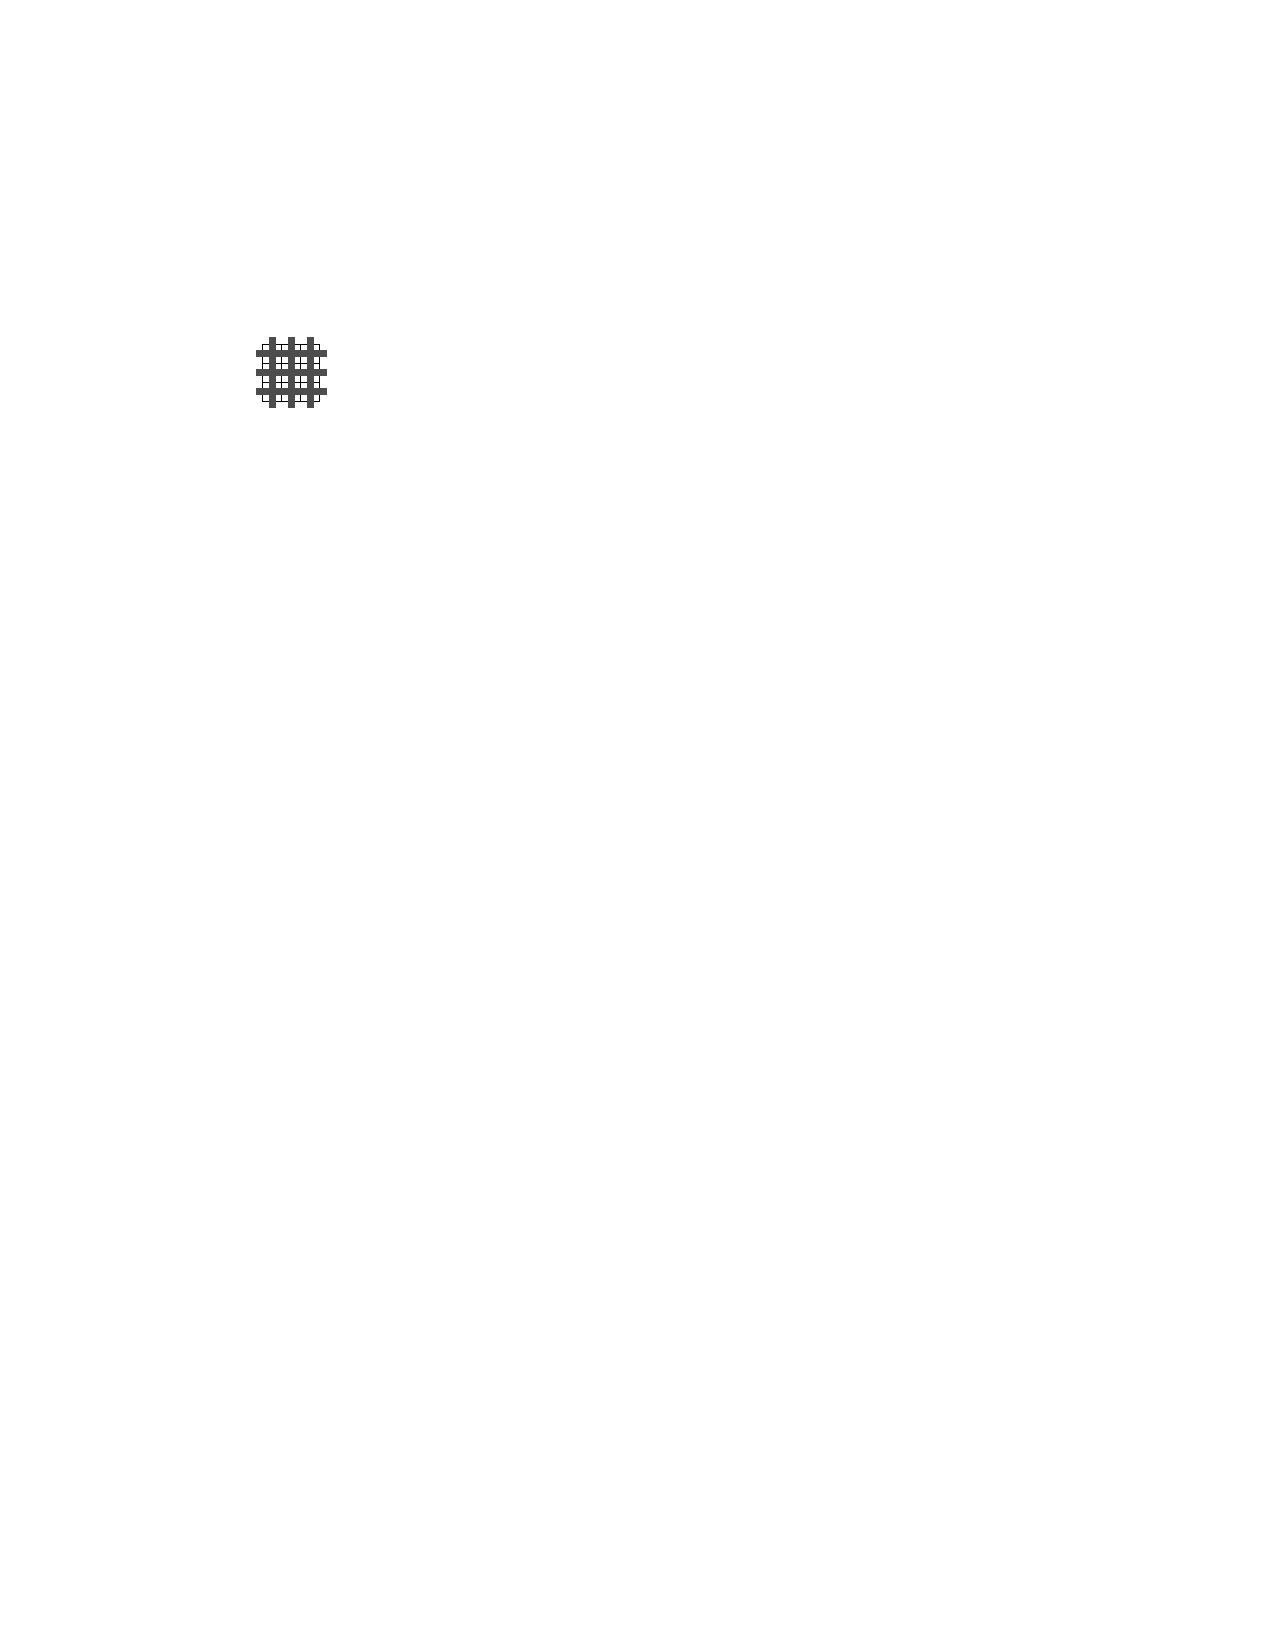
\includegraphics{misc/missing6}
\caption{\textit{Missing(6)} model}
\label{fig:missing6}
\end{figure}

An interesting observation is that the two most performant models also have the same number of backtracks. One of them is the model with nothing but channeling constraints, the other uses the \href{http://eclipseclp.org/doc/bips/lib/ic_global/occurrences-3.html}{\texttt{occurrences/3}} constraint which enforces arc-consistency. The first will detect when for a given \textit{row-column}, \textit{row-value}, \textit{column-value} or \textit{block-value} combination only one possible \textit{value}, \textit{column}, \textit{row} or \textit{position} remains. It will remove this value, column, ... from the domains of the other primal or dual variables\footnote{The difference between unequality constraints and channeling is explained in more detail in \cite{article:channeling}. Adding unequalities to the implementation slows down the search procedure because the channeling constraints already do this propagation and more.}. The second does the same ; it can propagate unequalities when the domain of a variable is reduced to a singleton but also knows when a value can be put in only one particular cell of a row, column or block. It is probably slower because the constraint itself is more generic than reification constraints.\\\par

A model combining the classic viewpoint with the fourth dual model was set up. Number of backtracks and runtimes are displayed in table \ref{tab:res2}.

\begin{snippet}[H]
\caption{Channeling constraints for the combined viewpoint model}\label{channeling}
\small
(multifor([Row,Column,Value], 1, N), param(Primal, Dual, K) do \\
    \qquad\#=(Primal[Row,Column], Value, Bool), \% reification \\
    \qquad block(K, Row, Column, Block), \% calls utility function to convert $R\times C\rightarrow B$ \\
    \qquad position(K, Row, Column, Position), \% calls utility function to convert $R\times C\rightarrow P$ \\
    \qquad\#=(Dual[Block,Value], Position, Bool) \% reification\\
)
\end{snippet}

The \texttt{first\_fail} heuristic generally outperforms \texttt{input\_order}. It considers variables with the smallest domain first, rather than considering variables in the order they were given. This increases pruning power as removing a value from the domain will remove a bigger part of the search tree because the branching count increases as you go down the tree (which is not necessarily the case when using \texttt{input\_order}). This tends to cause the number of backtracks to decrease. Unless the solution lies at the left side of the search tree generated by the \texttt{input\_order} heuristic performance will increase in comparison. \\\par

As for the \texttt{all\_different} constraints, more constraint propagation can be done when making use of \texttt{ic\_global} since it enforces bounds consistency rather than enforcing arc-consistency on the corresponding inequalities. This decreases the number of backtracks for every puzzle but may increase runtime for some of them (such as \textit{sudowiki\_nb49}) because the propagation takes time. The global constraints do tend to perform a little better on average (about 11.2 versus 11.5 seconds total runtime).

\subsection{CHR}

Some of the viewpoints considered previously were implemented in \texttt{CHR}, too. The runtimes are shown in table \ref{tab:res4}. The \texttt{first\_fail} variable heuristic and the \texttt{indomain\_min} value heuristic. These are easy to implement and generally perform quite nicely. The combined model generally performed at least as well as the worst of the two other models except when runtime was already low. This is to be expected ; the running times\\\par 

Because the channeling-only viewpoint performed best in ECLiPSe an attempt was made at implementing it in \texttt{CHR}. \\\par 

Due to a failed experiment\footnote{At some point a constraint \texttt{pos/4} was used to convert from \textit{row-column} combinations to the corresponding blocks and positions (e.g. \texttt{pos(2,3,1,6)}. This slowed down the algorithm a lot.} the focus was laid on adding redundant constraint instead of changing the viewpoint.

\newpage
\begin{table}[h]
\footnotesize
\bgroup
\def\arraystretch{1.3}
\begin{tabular}{ccccccccc}
\multicolumn{1}{l}{} & classic & dual1 & dual2 & dual3 & boolean & laburthe & member & channeling \\ \hline
Total/Average & 1981/142 & 2694/193 & 3467/248 & 2178/156 & 1998/143 & 14270/1020 & 1267/91 & 688/50 \\
Total/Average (minimum) & 2628/27 & 3183/32 & 3148/32 & 2612/27 & 2715/27 & 59340/594 & 1909/20 & 2026/20
\end{tabular}
\egroup
\caption{Runtimes for the various viewpoints (ECLiPSe) - shown in milliseconds. The \texttt{first\_fail + indomain\_min} heuristics were used.}
\label{tab:res1}
\end{table}

%\setlength\arrayrulewidth{0.5pt}
%\taburulecolor{gray}
\begin{table}[H]
\footnotesize
\bgroup
\def\arraystretch{1.3}
\begin{tabular}{ccc|cc}
\multicolumn{1}{l}{}    & \texttt{input\_order} & \texttt{first\_fail} & \texttt{input\_order} (global) & \texttt{first\_fail} (global) \\ \hline
& classic - dual & classic - dual & classic - dual & classic - dual \\
\textit{lambda} & 495/4712 - 162/1715 &  149/977 - 72/523 &  22/3 - 17/0 & 22/3 - 19/0 \\
\textit{hard17} & 132/873 - 87/389 & 92/419  - 68/198 &  20/1 - 27/1 & 27/1 - 29/1 \\
\textit{eastermonster}  & 62/119 - 75/125 & 58/101 - 84/155 &  237/51 - 236/49 & 169/33 - 256/66  \\
\textit{tarek\_052}  & 72/193 - 68/200 & 62/130 - 59/137 &  370/61 - 324/63 & 224/35 - 180/34  \\
\textit{goldennugget} & 103/520 - 98/441 & 87/358 - 90/281 &  687/104 - 517/72 & 334/76 - 264/44  \\
\textit{coloin} & 368/2209 - 246/2288 & 61/83 - 55/80 &  249/88 - 675/194 & 79/8 - 63/10  \\
\textit{extra2} & 305/4652 - 172/2894 & 641/7690 - 392/4232 &  18/0 - 18/0 & 19/0 - 21/0  \\
\textit{extra3} & 530/4712 - 176/1715 & 166/977 - 93/523 &  22/3 - 17/0 & 22/3 - 19/0   \\
\textit{extra4} & 1445/15116 - 409/6087 & 234/2097 - 139/1031 &  23/4 - 19/0 & 22/3 - 19/0  \\
\textit{inkara2012} & 21/50 - 49/72 & 91/273 - 75/199 &  42/3 - 97/3 & 97/17 - 106/15  \\
\textit{clue18} & 220/1838 - 161/1977 & 93/439 - 96/493 &  272/69 - 207/47 & 12/8 - 62/6  \\
\textit{clue17} & 523/5520 - 329/3509 & 78/270 - 72/201 &  17/0 - 18/0 & 22/0 - 18/0  \\
\textit{sudowiki\_nb28} & 324/2851 - 501/4555 & 322/2221 - 455/3015 & 1083/413 - 1292/421 & 638/297 - 875/353  \\
\textit{sudowiki\_nb49} & 186/1078 - 127/749 & 88/655 - 137/672 & 246/48 - 201/40 & 224/58 - 275/62  \\\hline
Total/Average (ms) & 4782/342 - 2654/190 & 2216/159 - 1880/135 & 3302/236 - 3660/262 & 2013/144 - 2201/157   \\
Total/Average (backtracks) & 44443/3175 - 26716/1909 & 16690/1192 - 11740/838 & 848/61 - 890/64 & 542/39 - 591/42                          
\end{tabular}
\egroup
\caption{Results for the classic and alternative \texttt{dual4} viewpoint (ECLiPSe) - shown as milliseconds/backtracks. In both models the \texttt{input\_order} heuristic outperforms \texttt{first\_fail} for puzzle \textit{extra2}. This is because the latter tends to direct the search \textit{`down the wrong alleys'} hence the relatively large number of backtracks. Since the constraints are the same the runtime increases proportionally.}
\label{tab:res2}
\end{table}

\begin{table}[H]
\centering
\footnotesize
\bgroup
\def\arraystretch{1.3}
\begin{tabular}{ccc|cc}
\multicolumn{1}{l}{}    & \texttt{input\_order} & \texttt{first\_fail} & \texttt{input\_order} (global) & \texttt{first\_fail} (global) \\ \hline
\textit{lambda} & 160/507 & 122/188 & 29/3 & 36/3 \\
\textit{hard17}  & 138/264 & 116/155 & 26/1 & 36/1 \\
\textit{eastermonster} & 79/102 & 163/218 & 351/51 & 395/78 \\
\textit{tarek\_052} & 137/170 & 137/136 & 625/61 & 219/39 \\
\textit{goldennugget} & 217/286 & 50/10 & 1261/104 & 30/0 \\
\textit{coloin} & 381/1009 & 55/19 & 363/87 & 67/8 \\
\textit{extra2} & 115/263 & 120/253 & 25/0 & 28/0 \\
\textit{extra3} & 152/507 & 113/188 & 32/3 & 60/3 \\
\textit{extra4} & 266/1111 & 153/330 & 40/4 & 38/3 \\
\textit{inkara2012} & 36/36 & 201/177 & 54/3 & 131/19 \\
\textit{clue18} & 37/730 & 90/62 & 351/69 & 71/8 \\
\textit{clue17} & 182/462 & 40/1 & 24/0 & 24/0 \\
\textit{sudowiki\_nb28} & 866/2581 & 400/713 & 1667/412 & 247/60 \\
\textit{sudowiki\_nb49} & 3369/564 & 17/252 & 287/49 & 198/46 \\\hline
Total/Average (ms) & 3369/241 & 1918/137 & 5127/37 & 1575/198 \\
Total/Average (backtracks) & 8592/613 & 2702/193 & 847/61 & 268/19
\end{tabular}
\egroup
\caption{Results for the combined (classic + \texttt{dual4}) viewpoint (ECLiPSe) - shown as milliseconds/backtracks.}
\label{tab:res3}
\end{table}

\begin{table}[H]
\footnotesize
\centering
\bgroup
\def\arraystretch{1.3}
\begin{tabular}{cccc|cc}
\multicolumn{1}{l}{} & classic & dual & combined & channeling-only & dual (bis) \\ \hline
\textit{lambda} & 0 & 0 & 0 & 0 & 0  \\
\textit{hard17} & 0 & 0 & 0 & 0 & 0  \\
\textit{eastermonster} & 0 & 0 & 0 & 0 & 0  \\
\textit{tarek\_052} & 0 & 0 & 0 & 0 & 0  \\
\textit{goldennugget} & 0 & 0 & 0 & 0 & 0  \\
\textit{coloin} & 0 & 0 & 0 & 0 & 0  \\
\textit{extra2} & 0 & 0 & 0 & 0 & 0  \\
\textit{extra3} & 0 & 0 & 0 & 0 & 0  \\
\textit{extra4} & 0 & 0 & 0 & 0 & 0  \\
\textit{inkara2012} & 0 & 0 & 0 & 0 & 0  \\
\textit{clue18} & 0 & 0 & 0 & 0 & 0  \\
\textit{clue17} & 0 & 0 & 0 & 0 & 0  \\
\textit{sudowiki\_nb28} & 0 & 0 & 0 & 0 & 0  \\
\textit{sudowiki\_nb49} & 0 & 0 & 0 & 0 & 0  \\\hline
Total/Average & 0 & 0 & 0 & 0 & 0  \\
Total/Average (minimum) & 0 & 0 & 0 & 0 & 0                      
\end{tabular}
\egroup
\caption{Results for the CHR Sudoku solver - shown as backtracks/milliseconds. Dual corresponds to \texttt{dual4} in the ECLiPSe version, dual (bis) with \texttt{dual3}.}
\label{tab:res4}
\end{table}